% !TEX root = root.tex
\chapter{\label{chap:snase}Mechanical Evolution of Interfacial Layers of SNase: The Role of Protein Conformation in Layer Formation}
\chaptermark{Protein Unfolding}

\section{Introduction}

Previous work by our group on the microrheology of the protein $\beta$-lactoglobulin layers\cite{Lee2010} supports a picture of layer formation through a gelation process, where proteins associate through intermolecular disulfide bonds. In Chapter \ref{chap:lysozyme}, my work applied similar techniques to layers of lysozyme in an effort to understand better those aspects of the viscoelastic transition in protein layers that are universal and those that are system specific. As discussed above, the lysozyme study supported a competing (though not completely mutually exclusive) picture of layer evolution in terms formation of a soft glass phase. One key difference between the $\beta$-lactoglobulin layers forming at the air--water interface and those of lysozyme was the prevalence of mesoscale heterogeneity during an extended stage of formation in the $\beta$-lactoglobulin. The sources of the differences in layer formation between these systems are difficult to identify. A key feature that generally may differ among different proteins, however, is the degree and type of conformational change that the proteins undergo on adsorbing and the stability of the protein against these changes. In this chapter we describe a study designed to isolate the role of protein conformation in the evolution of interfacial layers' mechanical response by exploiting a structural feature of the protein Staphylococcal nuclease (SNase). We studied layer formation by wild-type SNase---the protein as it is found in nature---which assumes a folded conformation for the solution conditions considered and an engineered variant sharing almost the same chemical composition but having a completely disordered, unfolded structure.

Changing one particular residue catastrophically destabilizes the folded structure of SNase. This sensitivity is due to a particular structural feature of SNase illustrated in the ribbon diagram in Figure \ref{fig:ribbon-diagram}. SNase exhibits a structural motif known as a beta barrel, a large beta-sheet that twists and coils to form a closed structure in which the first strand is hydrogen-bonded to the last. At one opening of this barrel, an $\alpha$-helix acts as a lid, keeping water from flooding the hydrophobic interior of the barrel. The helical structure of an $\alpha$-helix relies on a rotational degree of freedom common to all amino acids save one, proline, whose cyclic side chain lends it a distinctive structural rigidity. When an amino acid in the center of the $\alpha$-helix (at residue 62, which happens to be threonine) is replaced by proline, the arc of helix is kinked, effectively breaking the lid, exposing the hydrophobic interior of the beta barrel to water, and ruining the stability of the entire folded structure. Here, we describe comparative microrheology experiments on layers of wild-type and disordered SNase adsorbed to the air--water interface. From differences in the mechanical evolution of the layers formed by the two proteins, we speculate on the role of protein unfolding in the evolution of the mechanical response of the interface.

\begin{figure}
 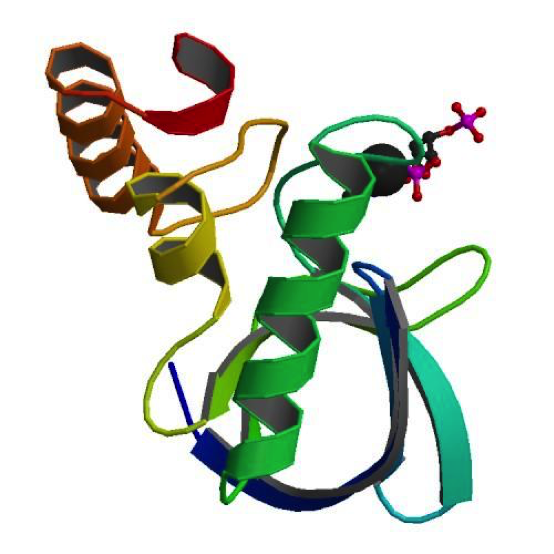
\includegraphics[width=\linewidth,keepaspectratio]{snase/ribbon-diagram}
 \caption[\lofimage{snase/ribbon-diagram}Ribbon diagram of Wild-Type SNase]{\label{fig:ribbon-diagram}This ribbon diagram shows the secondary structure of SNase. The $\alpha$-helix, positioned front and center from this perspective, acts a lid on the beta barrel (a beta sheet curved into a closed structure) beneath it. The interior of the beta barrel is hydrophobic, and the $\alpha$-helix helps keep water out. Change one residue in the middle of the helix creates a kink, effectively breaking the lid and ruining the stability of the folded structure.}
\end{figure}

\section{Experimental Methods}

\subsection{Protein Fabrication}

The disordered SNase was fabricated by our collaborators in the lab of Prof. Bertrand Garcia-Moreno E. using the polymerase chain reaction (PCR). PCR is a well established technique in biology, briefly reviewed here for interested readers. To manufacture protein with a certain engineered mutation, a fragment of DNA expressing the desired mutation is synthesized by chemically joining base pairs. This is a primer. A plasmid (circular ring of DNA) is obtained which largely compliments the fragment except at the site of the mutation. The primers and plasmids are combined in a soup of loose ribonucleotides and DNA polymerase, which marches along the chain and builds a DNA polymer along complemtary strands. The original primers are extended to full strands, and more full copies are made as the process proceeds. Finally, bacteria are made to imbibe the plasmids, and they manufacture mutated proteins in accordance with the mutated DNA. The product is purified and flash-frozen into droplet-sized beads for storage.

\subsection{Sample Preparation}

The frozen protein solution was thawed and diluted to 0.05 mg/ml in a 10 mM sodium phosphate buffer, pH 7.4. Then, following the protocol developed for the lysozyme study described in Chapter \ref{chap:lysozyme}, a volume of 0.5 ml was placed into a sample cell, where an air--water interface was formed. Colloidal probes were spread across the interface, dispersed in a solution of equal parts water and isopropyl alcohol.

\subsection{Active Microrheology}

The experiments focused on active microrheology measurements employing ferromagnetic Nickel nanowires using procedures like those described in detail in the previous chapters, wherein the wires' orientations are tracked following a 90$^\circ$ step change in the direction of an applied magnetic field. A total of 12 trails were conducted, 6 using wild-type SNase and 6 using the disordered variant. Measurements were performed as a function of age. Up to 15 separate wire rotations were performed at each age, using field strengths of 10--100 G, selected to match the stiffness of the layer so as to generate an observable wire rotation.


\section{Results}
\subsection{Wild-Type SNase Layer Evolution}

At early ages in the layer's evolution, the wild-type layers were always found to exert a simple viscous drag on the wire. The angle between the wire axis and the final field direction as a function of time was well described by Eq. (\ref{eq:sasha}),

\begin{equation*}
 \theta(t) = 2 \tan^{-1} \left[ \exp \left( -\frac{\mu B}{\zeta_r} (t-t_0) \right) \right].
\end{equation*}

\noindent where, as in Chapter \ref{chap:lysozyme}, $\mu$ is the wire's magnetic moment, $B$ is strength of the externally-applied magnetic field, $\zeta_r$ is a rotational drag coefficient, and $t_0$ is an experimental parameter that accounts for uncertainty in the time that the wire begins rotating in response to the field change. Figure \ref{fig:fitting-viscous-form}(a) shows rotational trajectories $\theta(t)$ for a wire of length $L=8.05$ \textmu m in a wild-type layer at age $t_a=13$ minutes under varied field strengths. Fitting Eq. (\ref{eq:sasha}) to each rotation gives a rate, $K=\mu B/\zeta_r$, which is plotted against field strength $B$ in Figure \ref{fig:fitting-viscous-form}(b). The rotational drag coefficient $\zeta_r$ can be extracted from the slope of linear regression to $K(B)$. Then, using Eq. (\ref{eq:wire_zeta}), $\zeta_r = 1.48 L^2\eta_s$, we obtain the interfacial viscosity $\eta_s$. Thus, several wire rotations performed in succession at roughly the same age $t_a$ are reduced to a single number characterizing the linear shear rheology of the layer at that age. Figure \ref{fig:wt-viscosity-with-age} shows how, in several identically-prepared trials of wild-type SNase, the viscosity increased exponentially with the age of the layer over a wide range of ages. The least-squared best fit of an exponential, $\eta_s=\eta_{s,0}\, e^{\Gamma t}$, to this data is also shown, and it gives $\Gamma=1.41 \pm 0.05 \times 10^{-5}$ s$^{-1}$ and $\eta_{s,0}=0.10 \pm 0.2$ \textmu Pa$\cdot$m$\cdot$s. (The Boussinesq number for this interfacial viscosity are wire length is 12.) At ages later than those represented in this figure, the wire rotations changed qualitatively in a way that could no longer be explained in terms of simple viscous drag.

Figures \ref{fig:deviation-shear-thinning} and \ref{fig:deviation-elastic-jump} show two kinds of deviation from viscous response that were observed. Figure \ref{fig:deviation-shear-thinning}, shown with a best-fit viscous form, turns more quickly through the middle of its rotation than can be explained by viscous drag, which is suggestive of shear-thinning and qualitatively similar to the power-law fluid behavior shown previously in Figure \ref{fig:early-and-late-rotation}(b). The second example, in Figure \ref{fig:deviation-elastic-jump}, shows what appears to be an elastic jump at the beginning of the rotation as the layer yields. More detailed analysis would be needed to see whether this indeed holds. Future work will apply the analysis of Chapter \ref{chap:lysozyme} to this data.

   \begin{figure}
    \centering
    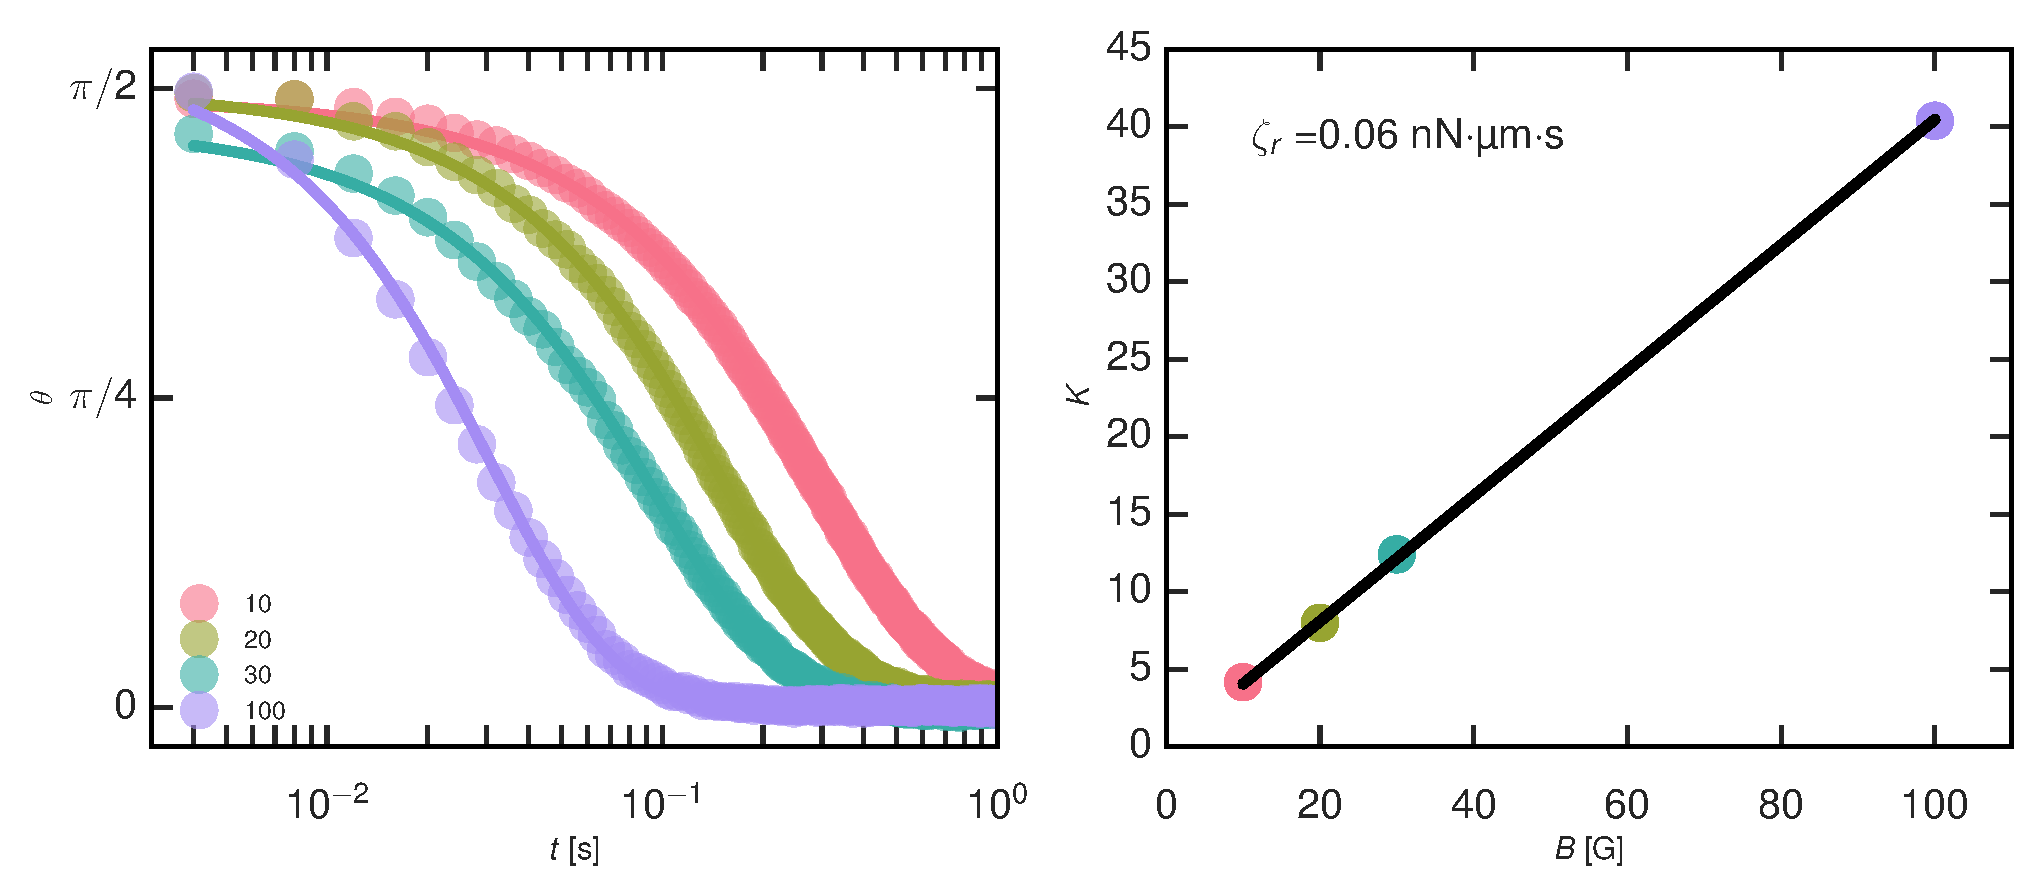
\includegraphics[width=\columnwidth]{snase/fitting-viscous-form} % from AT49 V5.ipynb
    \caption[Rotational viscous drag on a nanowire extracted from rotational tragictories]{\label{fig:fitting-viscous-form}(a) Rotational trajectories $\theta(t)$ of a wire in a wild-type SNase layer at age $t_a=13$ minutes under a 90$^\circ$ step change in magnetic field direction, under varied field strengths. Eq. \ref{eq:sasha} is fit to each rotation, giving a rate $K=\mu B/\zeta_r$, which is plotted against field strength $B$ in (b). The slope of the linear regression to this data is used to compute $\zeta_r$.}
    \end{figure}

   \begin{figure}
    \centering
    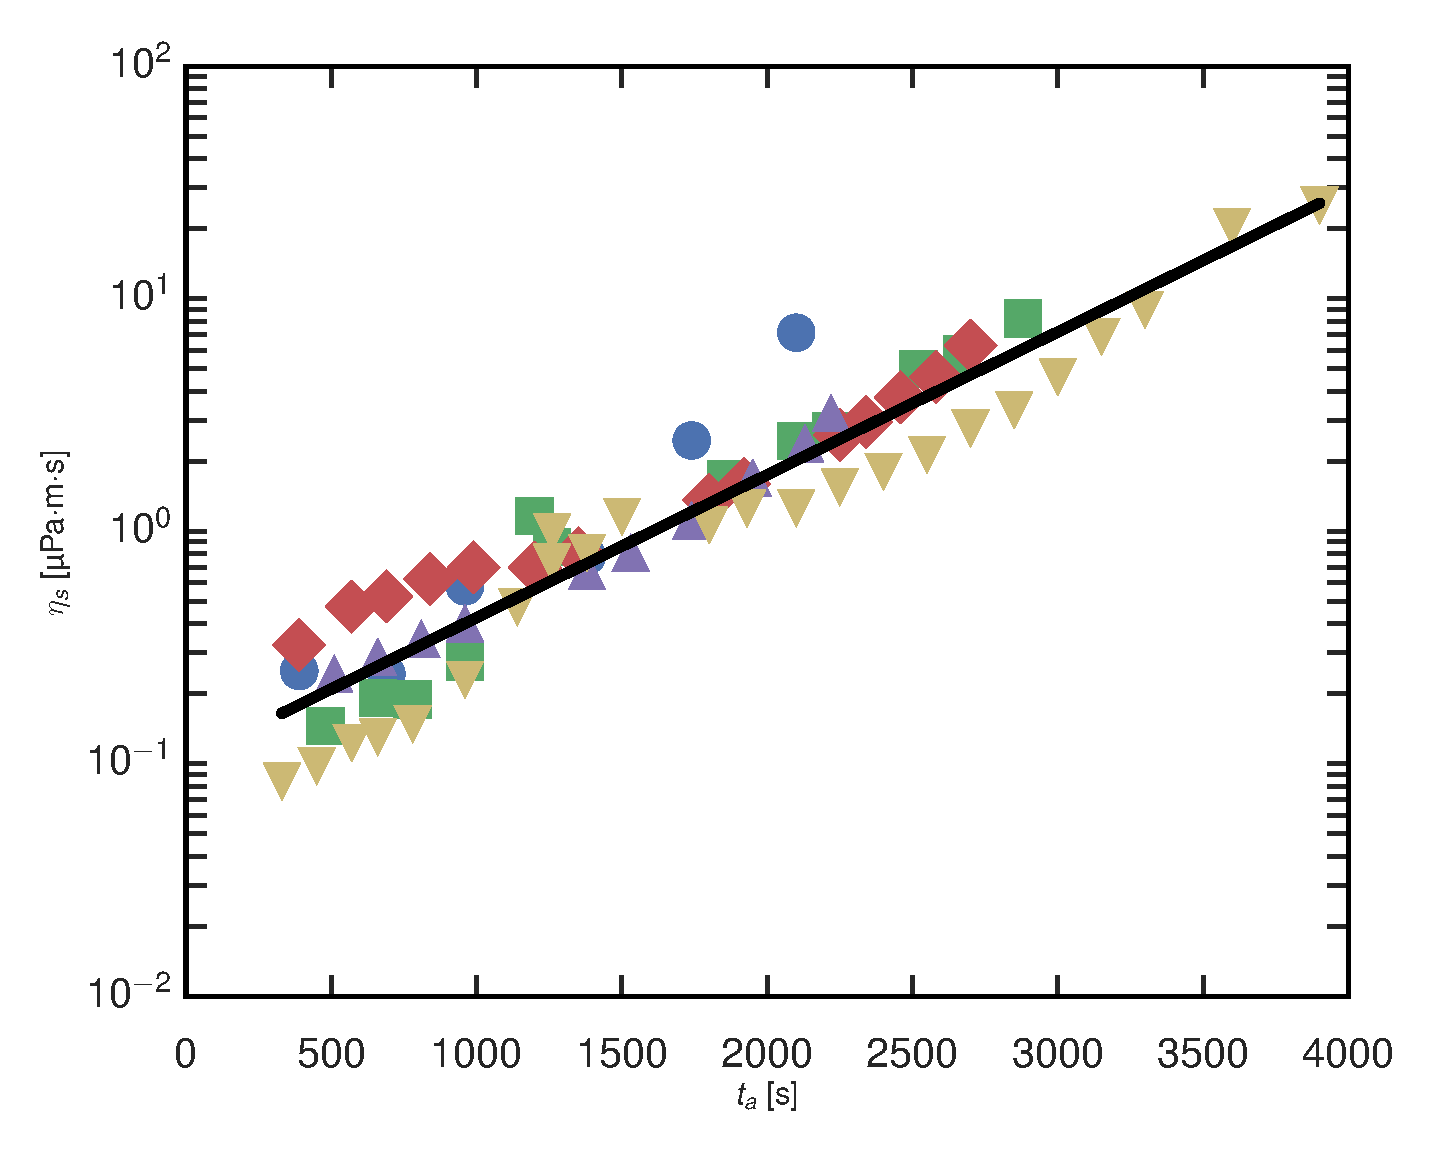
\includegraphics[width=\columnwidth]{snase/wt-viscosity-with-age}
    \caption[The interfacial viscosity of a wild-type SNase layer as a function of layer age.]{\label{fig:wt-viscosity-with-age}The interfacial viscosity of a wild-type SNase layer, computed from wire rotation curves like those in Figure \ref{fig:fitting-viscous-form}, rose exponentially with layer age $t_a$. The black line shows an exponential best fit to the data, given in the text. Data from several identically-prepared trails are shown, differentiated by plot markers.}
    \end{figure}
    
\begin{figure}
    \centering
    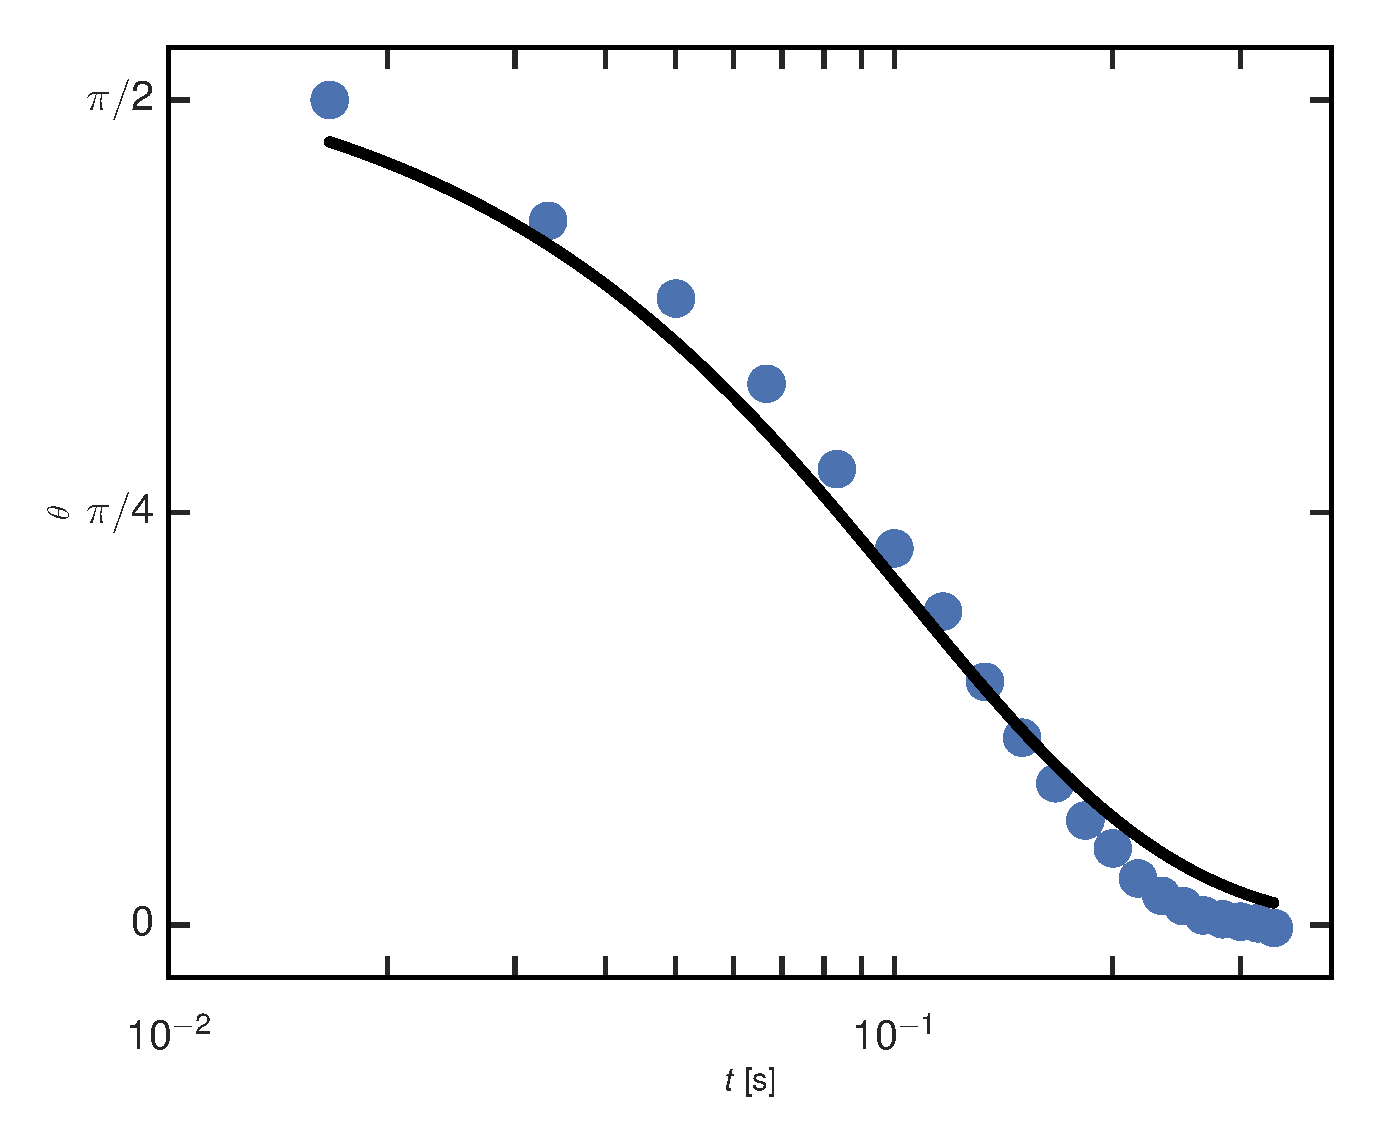
\includegraphics[width=\columnwidth]{snase/shear-thinning} % from AT41 V13
    \caption[A wire rotation in a disordered SNase layer that cannot be well described by a viscous response.]{\label{fig:deviation-shear-thinning}This rotation, performed under 100 G in a layer of disordered SNase aged 2 hours, cannot be well described by a viscous response. The wire turns more quickly during the middle of its rotation, which is suggestive of shear-thinning and is qualitatively similar to power-law fluid behavior, as described in the text.}
    \end{figure}
    
\begin{figure}
    \centering
    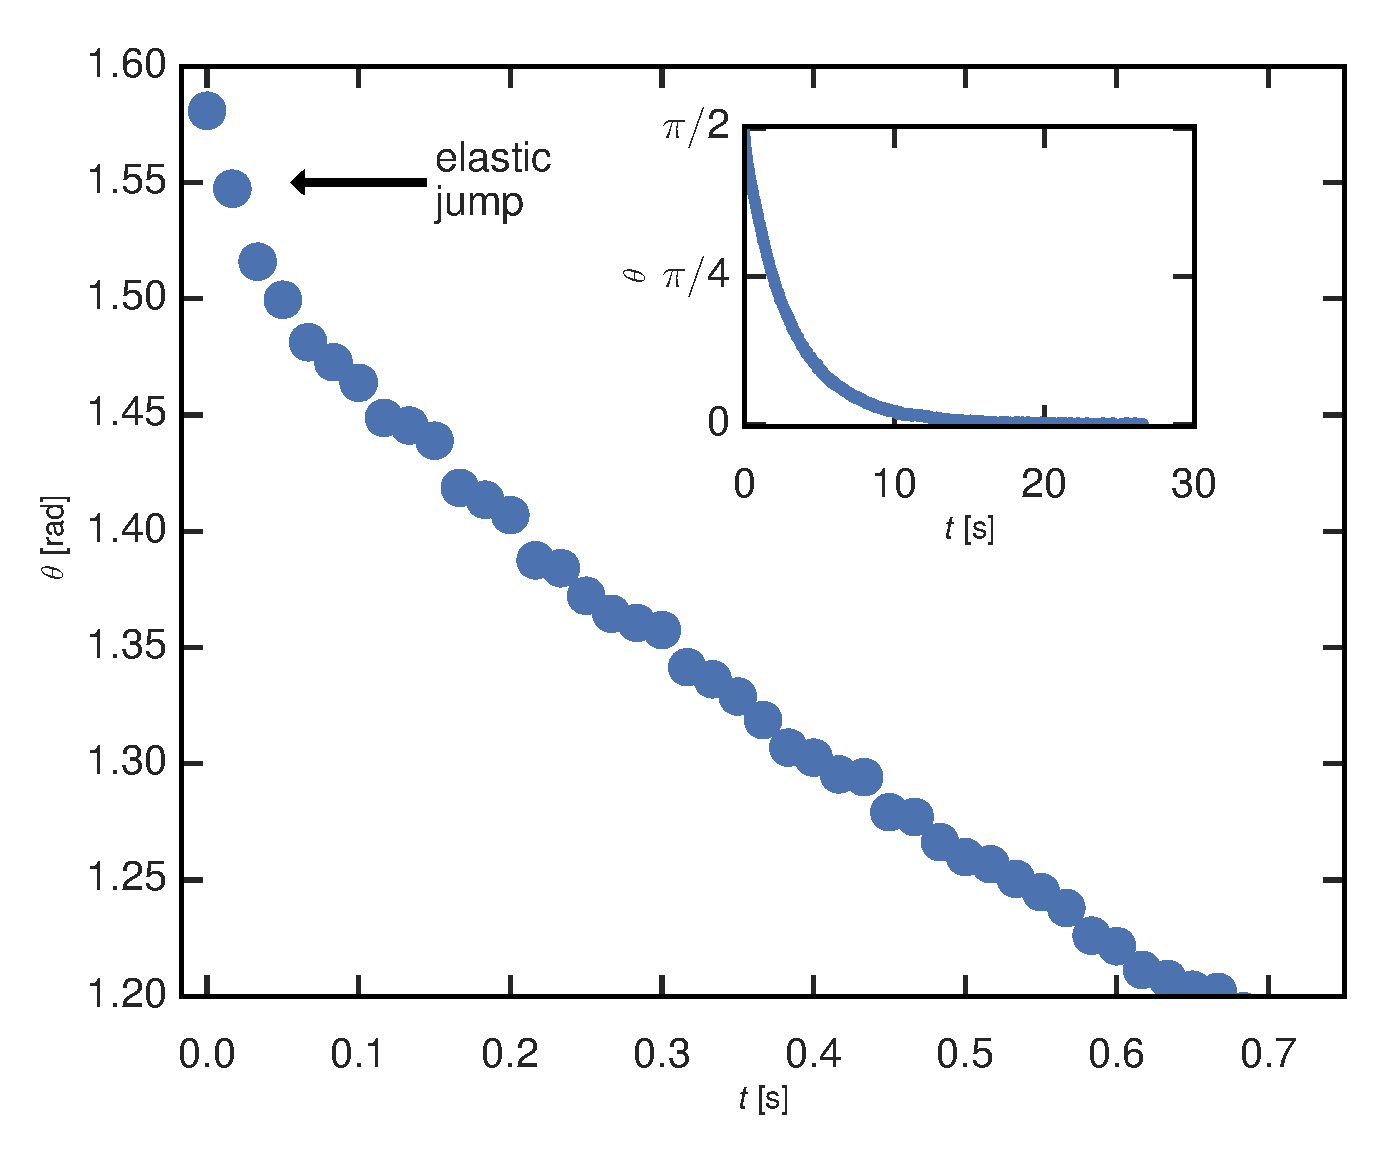
\includegraphics[width=\columnwidth]{snase/elastic-jump} % from AT410 V14
    \caption[Another wire rotation in a disordered SNase layer that cannot be well described by a viscous response.]{\label{fig:deviation-elastic-jump}In this rotation, also performed under 100 G in a layer of disordered SNase aged 2 hours, the layer appears to yield quickly to the initial torque, evincing a mostly elastic response followed by a more liquid-like response as the wire completes a full 90$^\circ$ rotation. (It does not recoil.)}
    \end{figure}
   

\subsection{Disordered SNase Layer Evolution}

In contrast to the wild-type layers whose microrheology showed strong trial-to-trial reproducibility, the wire rotations in layers of disordered SNase showed considerable trail-to-trail variation. Measurements in three of the six trials could be well-described by viscous drag at early ages, as in the wild-type trials. The others showed a more complex response from the beginning. The interfacial viscosities of those showing viscous behavior are plotted in Figure \ref{fig:dis-viscosity-with-age}. The change in viscosity is much less pronounced and occurs more slowly than in wild-type layers. The magnitudes of the viscosity in the disordered layers also shows more variability among different trials. (To aid the comparison, note that Figures \ref{fig:wt-viscosity-with-age} and \ref{fig:dis-viscosity-with-age} are plotted on the same scale and that the fit to the data in Fig. \ref{fig:wt-viscosity-with-age} is shown alongside the data in Fig. \ref{fig:dis-viscosity-with-age}.)

This apparent variability between trials of layer formation by disordered SNase may actually be a proxy for spatial variability in the layers. Straight, unaggregated wires are sufficiently sparse, and the evolution of the layer sufficiently fast, that it is not practical to observe more than one or two different wires in a given trial. Once a one or two usable wires are located in the layer, they must be carefully followed, and there is no time to locate an ensemble of wires and regions to compare before the layer has aged dramatically. Thus, we speculate that the layers generated by disordered SNase exhibit mesoscale (or larger) spatial heterogeneity that is not directly captured in the active microrheology measurements. Complementary passive microrheology measurements on ensembles of spheres could provide support for this picture.

   \begin{figure}
    \centering
    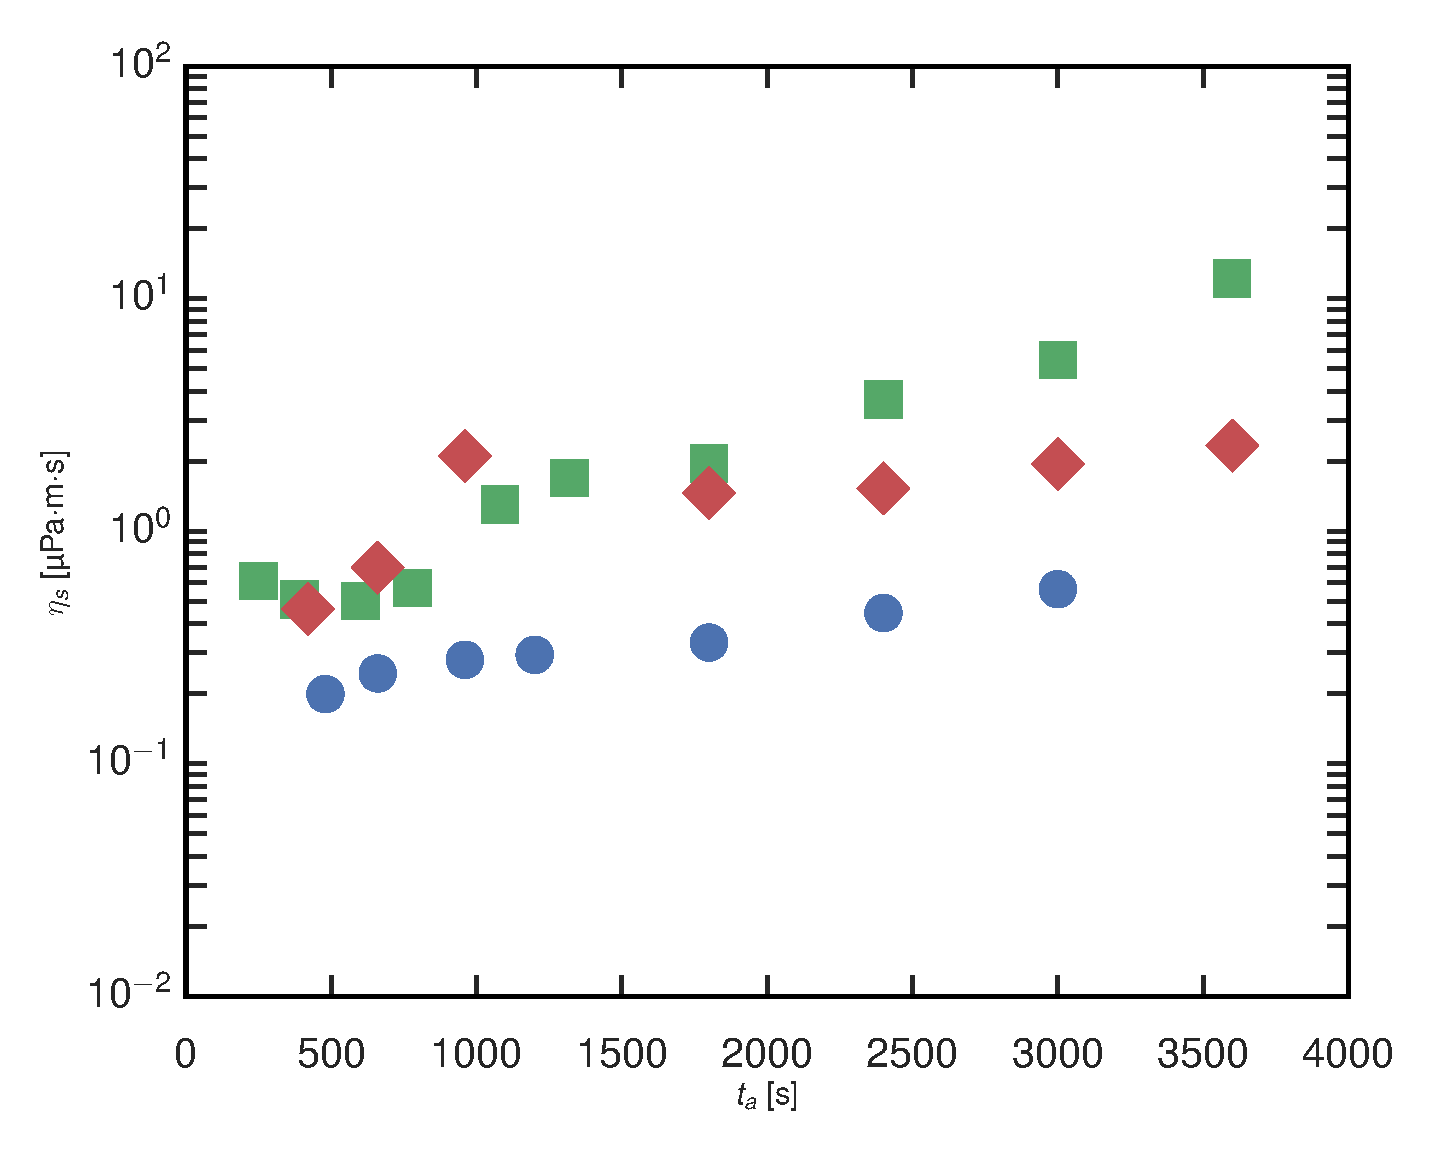
\includegraphics[width=\columnwidth]{snase/dis-viscosity-with-age}
    \caption[The interfacial viscosity of a disordered SNase layer as a function of layer age.]{\label{fig:dis-viscosity-with-age}In some trials or regions of a disordered SNase layer, the layer exerted viscous drag on a rotating wire with a viscosity that rose slowly in a way that can plausibly be interpreted as a weak power-law dependence on layer age. Compare to the much more dramatic and robust exponential increase exhibited by wild-type SNase in Figure \ref{fig:wt-viscosity-with-age}. The best-fit line from \emph{that} figure is shown here in gray for comparison. Data from several identically-prepared trails are shown, differentiated by plot markers. As noted in the text, some trials or regions of disordered SNase layers never exhibited viscous behavior.}
    \end{figure}


\section{Discussion \& Conclusion}

This comparative study of wild-type and disordered SNase has revealed how protein conformation in the bulk can play a dramatic role in the evolution of an interfacial layer's mechanical response during its formation. The weak age-dependence and strong variability observed in disordered films, which we associate with mesoscale spatial heterogeneity that sets in at very early ages, suggests a layer-formation process that is far from equilibrium. In contrast, the reproducible, steadily evolving, and apparently homogeneous layers formed by the wild type suggests a formation process in which the system has the opportunity to anneal. One possibility is that slow unfolding of the wild type at the interface introduces a rate-limiting step that allows the layer to acquire homogenous, dense coverage (leading to large viscosities) before non-viscous behavior, driven by protein association, sets in.